\documentclass{simplefamos}
\usepackage[danish]{babel} 
\usepackage{tikz}

% Specielle pakker/makroer til din artikel indl�ses her
% I dette eksempel benyttes f�lgende:
\newcommand{\makropakke}[1]{{\normalfont\ttfamily\bfseries #1}}
\newcommand{\AmSLaTeX}{{\protect\the\textfont2 A}
  \kern-.1667em\lower.5ex\hbox {\protect\the\textfont2 M}
  \kern-.125em{\protect\the\textfont2 S}-\LaTeX}

\begin{document}

\famosarticle{Side 9 S�tningen}{$\textbf{M}_3$-$\textbf{N}_5$ s�tningen}{Et dyk ned i gitterteorien}{Dan Saattrup Nielsen}{}
\famosprecistoc{$\textbf{M}_3$-$\textbf{N}_5$ s�tningen}

% Her begynder din artikel
I denne artikel vil det vise sig, hvordan gitre kan klassificeres som ikke-distributive ud fra gitterdiagrammet alene, et fascinerende resultat fundet af Birkhoff [3]. Det viser sig, at man blot skal tjekke, om et af de to nedenst�ende gitre $\textbf{M}_3$ eller $\textbf{N}_5$ kan indlejres i det p�g�ldende gitter.
\begin{center}
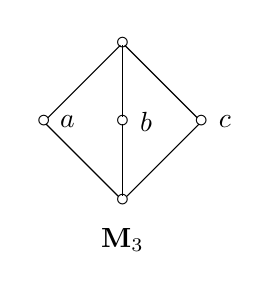
\begin{tikzpicture}
	\node (top) at (0,0) {$\circ$};
	\node (mid) [below of=top] {$\circ$};
	\node (left) [left of=mid] {$\circ$};
	\node (right) [right of=mid] {$\circ$};
	\node (bot) [below of=mid] {$\circ$};	
	\node (label) at (0,-2.5) {$\textbf{M}_3$};
	\node (a) at (-0.7,-1) {$a$};
	\node (b) at (0.3,-1) {$b$};
	\node (c) at (1.3,-1) {$c$};
	\draw[shorten >=-6pt,shorten <=-7pt] (top) -- (left);
	\draw[shorten >=-4pt,shorten <=-5pt] (top) -- (mid);
	\draw[shorten >=-6pt,shorten <=-7pt] (top) -- (right);
	\draw[shorten >=-6pt,shorten <=-7pt] (left) -- (bot);
	\draw[shorten >=-4pt,shorten <=-5pt] (mid) -- (bot);
	\draw[shorten >=-6pt,shorten <=-7pt] (right) -- (bot);
\end{tikzpicture}
\qquad
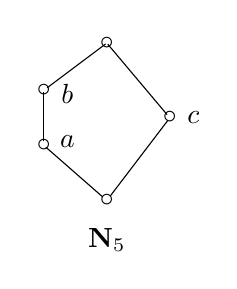
\begin{tikzpicture}
	\node (top) at (0,0) {$\circ$};
	\node (left1) at (-0.8,-0.6) {$\circ$};
	\node (left2) at (-0.8, -1.3) {$\circ$};
	\node (right) at (0.8,-0.95) {$\circ$};
	\node (bot) at (0,-2) {$\circ$};	
	\node (label) at (0,-2.5) {$\textbf{N}_5$};
	\node (a) at (-0.5,-1.25) {$a$};
	\node (b) at (-0.5,-0.65) {$b$};
	\node (c) at (1.1,-0.95) {$c$};
	\draw[shorten >=-6pt,shorten <=-7pt] (top) -- (left1);
	\draw[shorten >=-6pt,shorten <=-7pt] (top) -- (right);
	\draw[shorten >=-4pt,shorten <=-5pt] (left1) -- (left2);
	\draw[shorten >=-6pt,shorten <=-7pt] (left2) -- (bot);
	\draw[shorten >=-5pt,shorten <=-6pt] (right) -- (bot);
\end{tikzpicture}
\end{center}

Til at vise dette, skal der f�rst bruges et lemma omkring modul�re gitre:
\begin{lemma}
Et gitter \textbf{L} er ikke-modul�rt, hvis og kun hvis der findes et delgitter $\textbf{S}\leq\textbf{L}$ med $\textbf{N}_5\cong\textbf{S}$.
\end{lemma}
\begin{proof}
$'\Leftarrow'$: I $\textbf{N}_5$ ses det, hvor $a,b,c$ er defineret ift. relationerne angivet i ovenst�ende hassediagram, at $a\leq b$, men $a\lor(b\land c)\neq b\land(a\lor c)$, som medf�rer at $\textbf{N}_5$ er ikke-modul�rt. Dermed vil et gitter, med et delgitter isomorft til $\textbf{N}_5$, heller ikke v�re modul�rt.\\

$'\Rightarrow'$: Antag at $\textbf{L}$ ikke er modul�r. S� vil der findes $a,b,c\in L$, som opfylder $a\leq b$, men $a\lor(b\land c)<b\land (a\lor c)$. Lad $a_1:=a\lor(b\land c)$ og $b_1:=b\land(a\lor c)$. Da g�lder:
\begin{align*}
c\land b_1&=c\land(b\land(a\lor c))=c\land(c\lor a))\land b=c\land b\\
c\lor a_1&=c\lor(a\lor(b\land c))=(c\lor(c\land b))\lor a=c\lor a
\end{align*}

Da $c\land b\leq a\lor(b\land c)=a_1\leq b_1$ g�lder at $c\land b\leq c\land a_1\leq c\land b_1=c\land b$, som betyder at $c\land a_1=c\land b_1=c\land b$. Analogt g�lder at $c\lor b_1=c\lor a_1=c\lor a$. Det ses nu, at dette netop beskriver et gitter, isomorft til $\textbf{N}_5$, best�ende af $c$, $a_1$, $b_1$, $c\land a_1$ og $c\lor a_1$.
\end{proof}

S�tningen kan da formuleres som:
\begin{saetning}[$\textbf{M}_3$-$\textbf{N}_5$ s�tningen]
Et gitter \textbf{L} er ikke-distributivt, hvis og kun hvis der findes et delgitter $\textbf{S}\leq\textbf{L}$, med enten $\textbf{M}_3\cong \textbf{S}$ eller $\textbf{N}_5\cong\textbf{S}$.
\end{saetning}
\begin{proof}
$'\Leftarrow'$: Da det hverken for $\textbf{M}_3$ eller $\textbf{N}_5$ g�lder at $a\lor(b\land c)=(a\lor b)\land(a\lor c)$, er begge ikke-distributive og med samme argument som i beviset for Lemma 1 f�lger det, at $\textbf{L}$ er et ikke-distributivt gitter.\\

$'\Rightarrow'$: Antag at $\textbf{L}$ er ikke-distributivt og ikke indeholder en kopi af $\textbf{N}_5$ (da s�tningen ellers f�lger fra Lemma 1) - dermed kan det antages, uden tab af generalitet, at $\textbf{L}$ er modul�rt jf. Lemma 1. Der m� da findes elementer $a,b,c\in L$, som opfylder $(a\land b)\lor(a\land c)<a\land(b\lor c)$. Defin�r nu:
\begin{align*}
d&:=(a\land b)\lor(a\land c)\lor (b\land c)\\
e&:=(a\lor b)\land(a\lor c)\land (b\lor c)\\
a_1&:=(a\land e)\lor d\\
b_1&:=(b\land e)\lor d\\
c_1&:=(c\land e)\lor d.
\end{align*}

Det ses let, at $d\leq a_1,b_1,c_1\leq e$. Det vil vises at $d<e$. F�rst ses det fra absorptionsloven at
\begin{align*}
a\land e=a\land(b\lor c)
\end{align*}

og ved brug af den modul�re lov (bruges ved understregninger)
\begin{align*}
a\land d&=\underline{a}\land(\underline{(a\land b)\lor(a\land c)}\lor(b\land c))\\
&=((a\land b)\lor(a\land c))\lor(a\land(b\land c))\\
&=(a\land b)\lor(a\land c)
\end{align*}

f�lger det at $d<e$, ud fra ikke-distributivitetsantagelsen og den tidligere ulighed. Det vil nu vises, at diagrammet for $\textbf{L}$ indeholder en kopi af diagrammet for $\textbf{M}_3$, med $a=a_1$, $b=b_1$, $c=c_1$, bund $d$ og top $e$. For at vise dette, er det nok at vise at $a_1\land b_1=a_1\land c_1=b_1\land c_1=d$ og $a_1\lor b_1=a_1\lor c_1=b_1\lor c_1=e$. Vi viser at $a_1\land b_1=d$, resten forl�ber analogt. Modul�re lov understreges igen:
\begin{align*}
a_1\land b_1&=((a\land e)\lor\underline{d})\land(\underline{(b\land e)\lor d)}\\
&=((a\land e)\land((b\land\underline{e})\lor\underline{d}))\lor d\\
&=((a\land e)\land((b\lor d)\land e))\lor d\\
&=((a\land e)\land e\land(b\lor d))\lor d\\
&=((a\land e)\land(b\lor d))\lor d\\
&=(a\land\underline{(b\lor c)}\land(\underline{b}\lor(a\land c)))\lor d\\
&=(a\land(b\lor((b\lor c)\land(a\land c))))\lor d\\
&=(\underline{a}\land(b\lor\underline{(a\land c)}))\lor d\\
&=(a\land c)\lor(b\land a)\lor d\\
&=(a\land d)\lor d\\
&=d.
\end{align*}
\end{proof}

\begin{thebibliography}{9}
\bibitem[1]{amsldoc}{B.A Davey, H.A. Pristley. \textsl{Introduction to Lattices and Order, Second Edition}. Cambridge University Press, 2002.}
\bibitem[2]{amsldoc}{Stanley Burris, H.P. Sankappanavar. \textsl{A Course in Universal Algebra, Millenium Edition}. Springer-Verlag, 2009.}
\bibitem[3]{amsldoc}{Garrett Birkhoff. \textsl{Lattice Theory, Third Edition}. American Mathematical Society, Colloquium Publications, 1967.}
\end{thebibliography}

\end{document}
